\section{Results and Discussion}


\subsection{Rank epistasis correctly detects the absence of epistasis on a mixed additive/multiplicative landscape}

We find that rank epistasis correctly detects lack of epistasis on a deceptive additive and multiplicative fitness landscape where other metrics fail (Fig~\ref{fig:res:addmult}). 

Here, the additive model detects positive epistasis, since some sites are actually multiplicative. Under its baseline assumption, the whole genome appears epistatic because the average double-mutant has a much higher fitness than expected, due to the fact that some mutations are multiplied rather than summed. On the other hand, the multiplicative model detects negative epistasis, because some sites are actually additive. Under its baseline assumption, double-mutants have much lower fitness than expected, since some mutations are summed rather than multiplied.

Rank epistasis, however, correctly detects no epistasis across the entire genome. Rank epistasis does not assume additive or multiplicative interaction; it measures only relative perturbations in the rankings between single and double mutants. Without baseline assumptions, the metric is able to correctly determine that no epistasis is present in the genome, addressing a long-standing problem in detection of epistasis \citep{cordell_epistasis_2002, puniyani_meaning_2004}. 

\begin{figure}
    \centering
    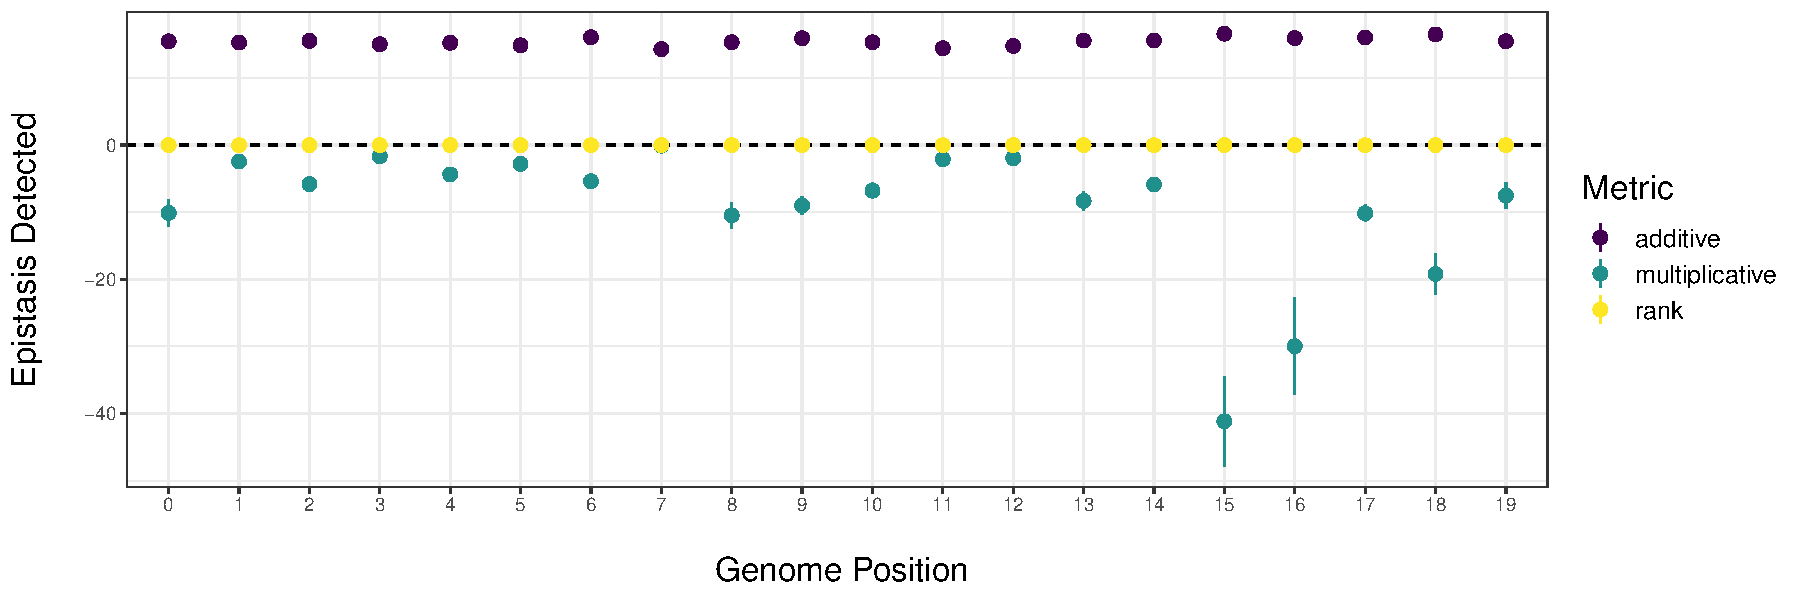
\includegraphics[width=\textwidth]{chapters/1-rank-epistasis/figs/summary_addmult.pdf}
    \caption{Comparison of rank epistasis metric to additive and multiplicative versions of metric $\epsilon$ as described in \cite{ostman_impact_2011}. Each x-axis tick represents one position in the genome, i.e., the $\epsilon$ or $\omega$ detected for that site. Note that $\epsilon$ and $\omega$ are not usually directly comparable; however, since $\omega=0$ and $\epsilon=0$ both indicate no epistasis, here $\omega$ is graphed on the same Y-axis. Dashed line at Y=0 indicates the true level of interactivity in genome. Dots represent mean and bars represent 95\% CIs for 100 replicates.}
    \label{fig:res:addmult}
\end{figure}

\subsection{Rank epistasis correlates with K on Canonical NK Landscapes}

\begin{figure}
    \centering
    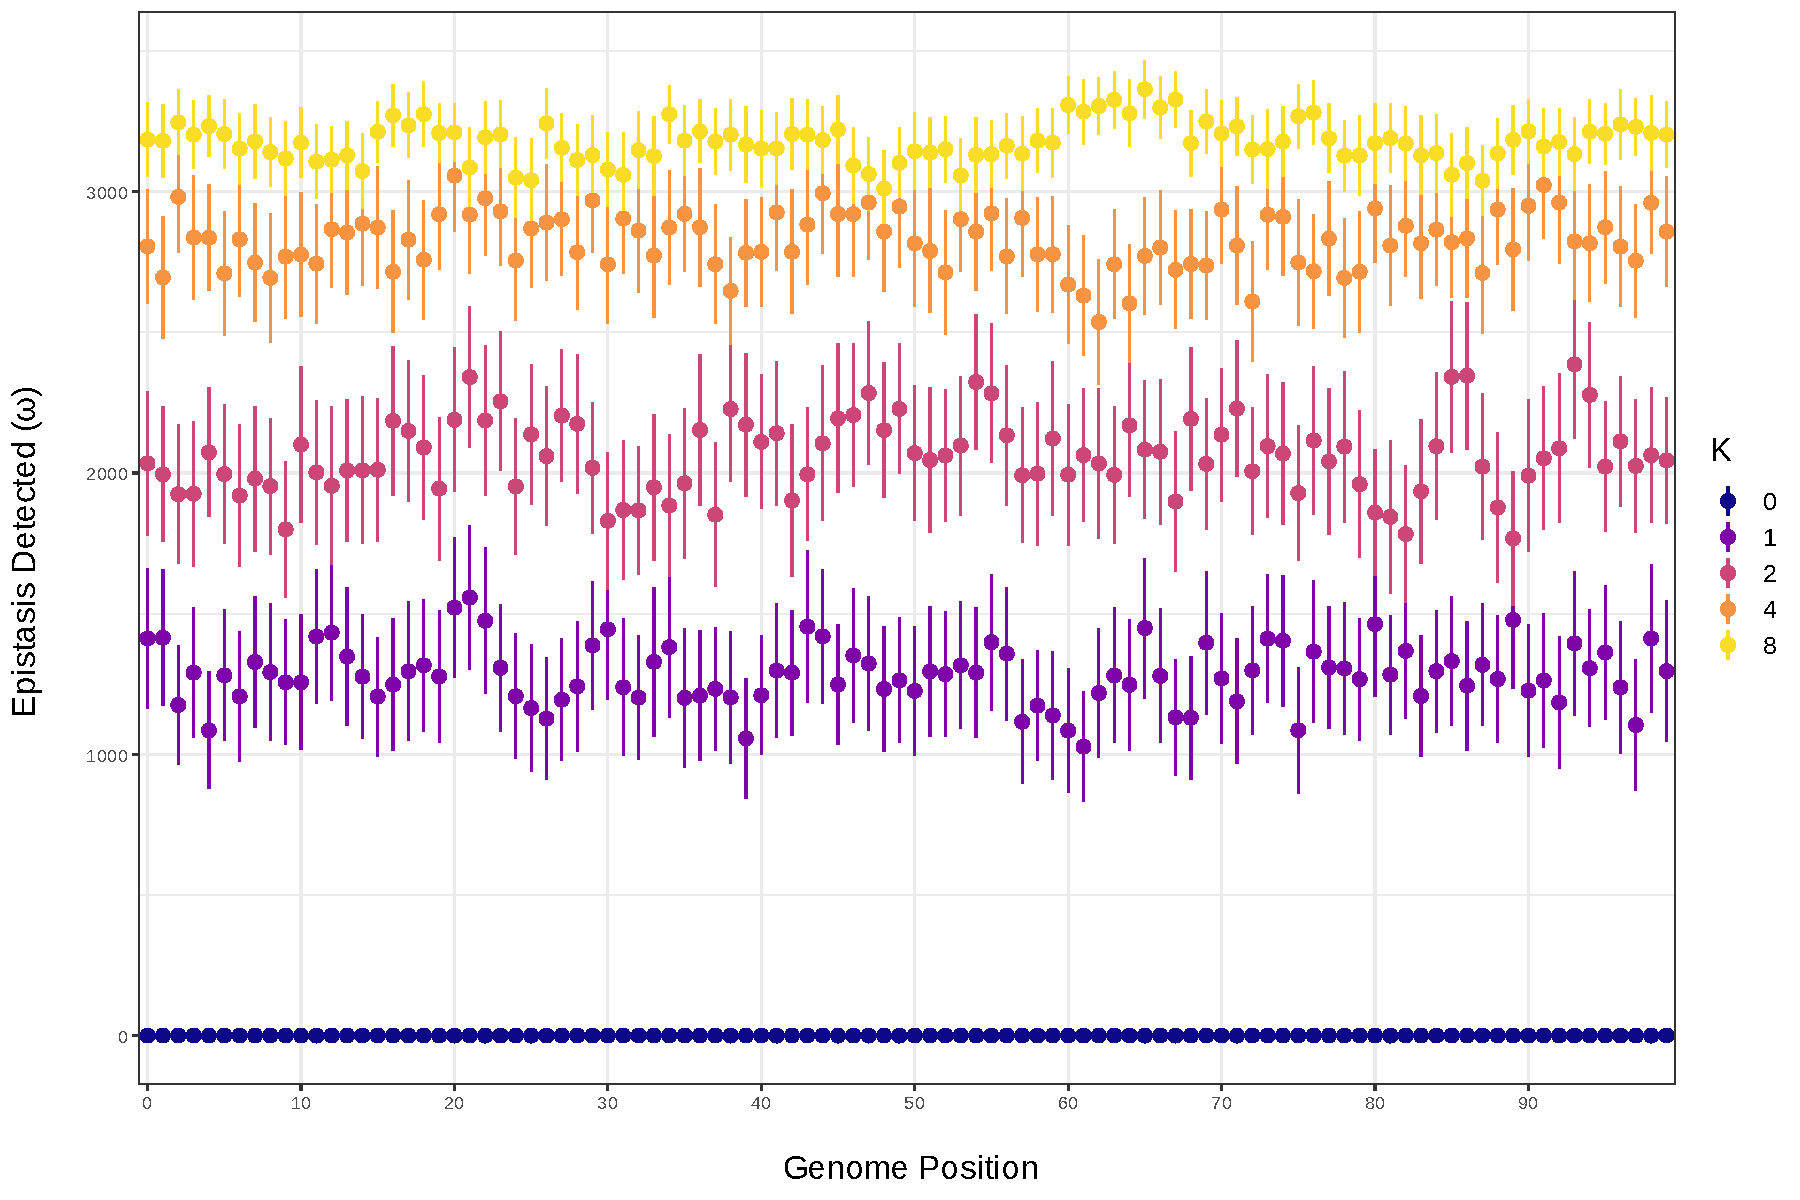
\includegraphics[width=\textwidth]{chapters/1-rank-epistasis/figs/summary_canon.pdf}
    \caption{Rank epistasis metric $\omega$ on a canonical NK landscape. Each x-axis tick represents one position in the genome, i.e., the $\omega$ detected for that site. Dots represent mean and bars represent 95\% CIs for 100 replicates.}
    \label{fig:res:canon}
\end{figure}

 On these landscapes, every site in a particular genome has the same degree of interactivity, so we expect roughly the same $\omega$ across sites. We also expect that identical landscapes with higher $K$ will generate a higher $\omega$. We find that the rank epistasis metric $\omega$ strongly correlates with $K$ when tested on traditional NK landscapes and correctly stratifies different values of $K$ when averaged across replicates (Fig.~\ref{fig:res:canon}). 

Of note is that $\omega$ and $K$ are not linearly correlated; for example, the average difference in measured $\omega$ from $K=0$ to $K=1$ is much larger than that from $K=1$ to $K=2$. In fact, as $K$ increases, the difference in $\omega$ between consecutive values of $K$ decreases.

One possible explanation for this effect is that the number of peaks in an NK landscape, and therefore the effect of perturbation on the genome, scales exponentially with $K$. In an NK landscape, each group of $K$ sites can take on $2^{K+1}$ possible fitness values. Therefore, for an NK landscape with $K=2$, each group of $K$ sites has $8$ possible fitness values, while each group in a landscape where $K=4$ has $32$ possible fitness values. NK landscapes therefore quickly reach a threshold where any mutation is likely to significantly change a genotype`s fitness; indeed, it has been shown that when $K>1$ it is exponentially difficult to find even local optima due to this effect \citep{kaznatcheev_computational_2019}.
Since rank epistasis is a measure of how perturbation affects the \textit{rank ordering} of possible mutants, genomes on NK landscapes quickly reach a point where they are close to maximally perturbed even at small $K$. This means the detected rank epistasis for $K=4$, for example, may not always be significantly different than for $K=8$ (see Fig~\ref{fig:res:canon}). Despite these limitations, on average rank epistasis is still able to distinguish low interactivity from high.

\subsection{Disentangling K on Variant NK Landscapes}

Rank epistasis successfully detects varying levels of per-site epistasis within the same genome on both variant landscapes, though the value of $\omega$ changes across genomes. In general, we find that rank epistasis on these variant landscapes produces a measure of \textit{apparent} epistasis. 

\begin{figure}
    \centering
    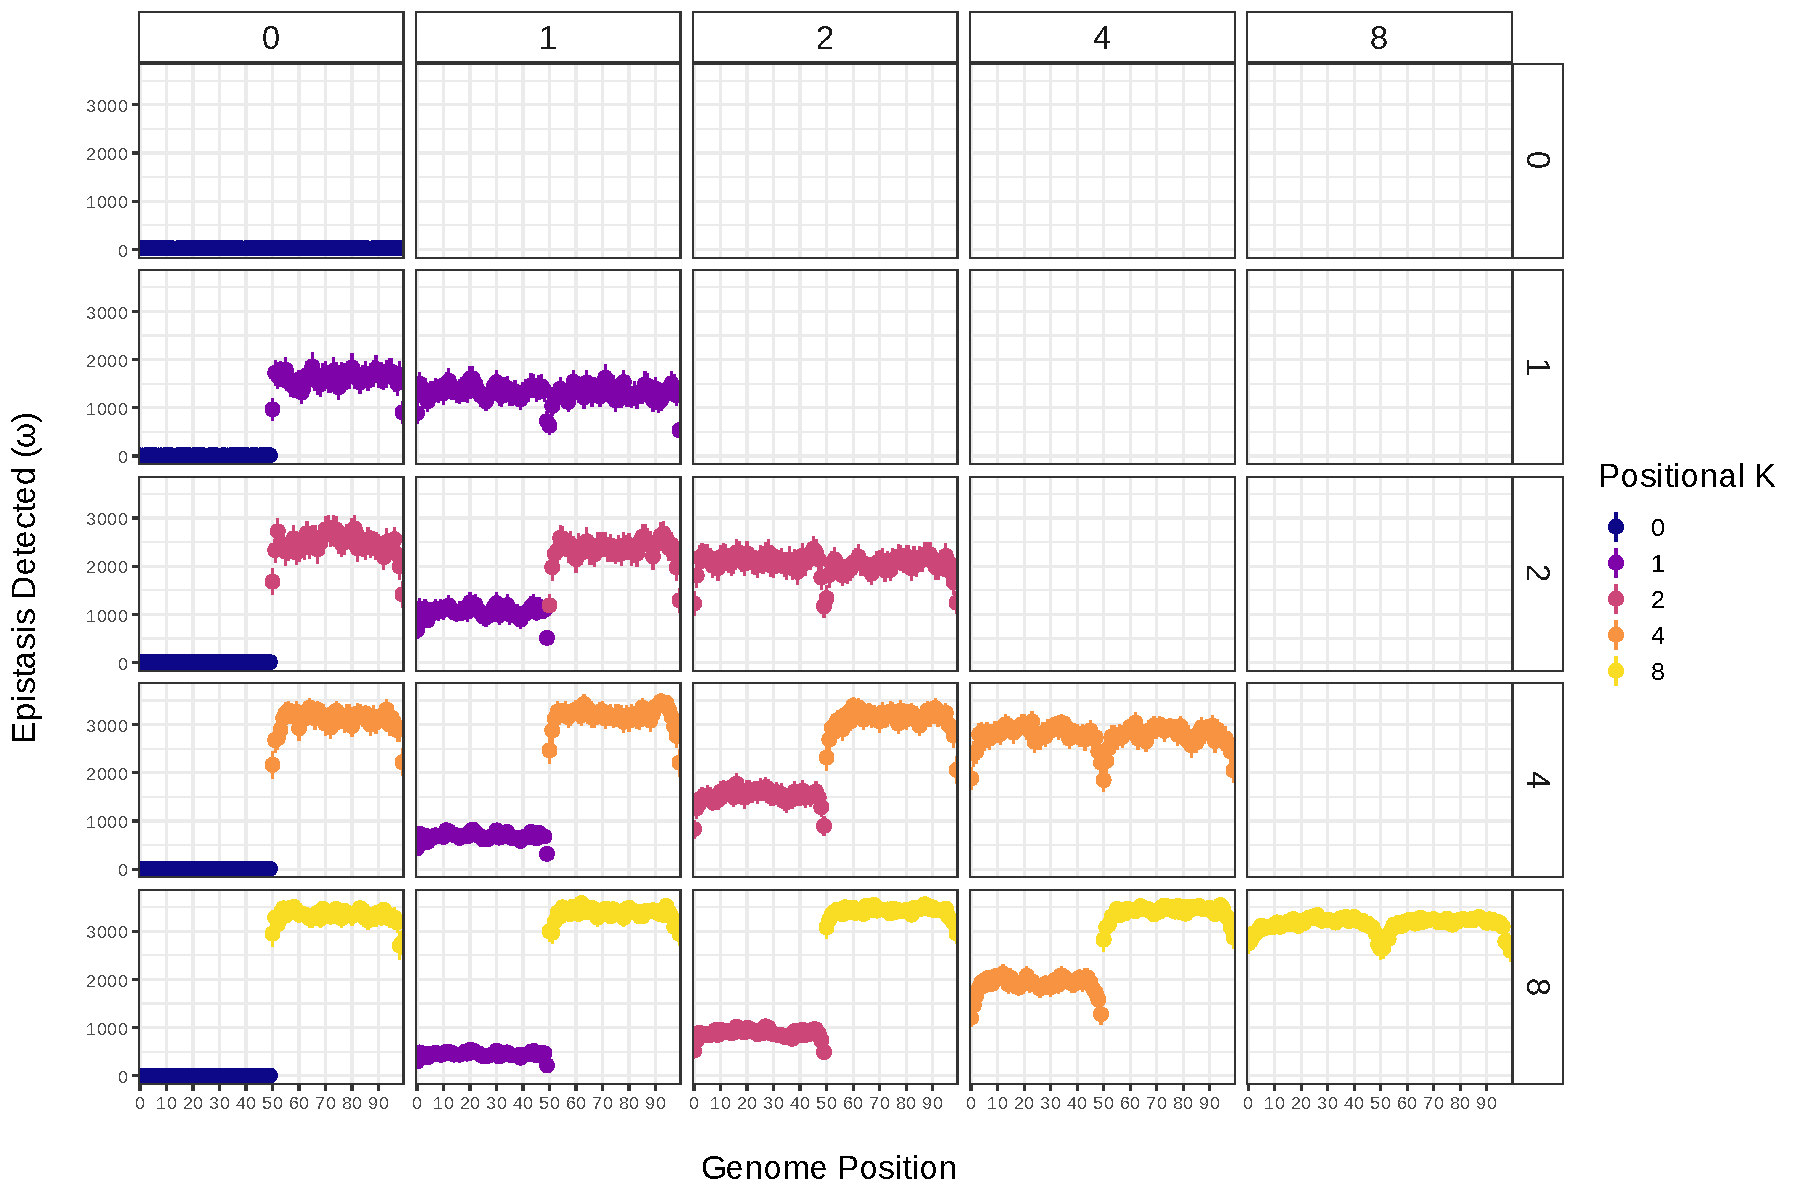
\includegraphics[width=\textwidth]{chapters/1-rank-epistasis/figs/summary_half.pdf}
    \caption{Rank epistasis metric $\omega$ on a Half-and-Half NK landscape. Top bars indicate the $K$ value set for the first $N=50$ values. Right bars indicate the $K$ value for the second $N=50$ values. Each x-axis tick within subplots represents one position in the genome, i.e., the $\omega$ detected for that site. Dots represent mean and bars represent 95\% CIs for 100 replicates.}
    \label{fig:res:half}
\end{figure}

\subsubsection{Rank epistasis measures different epistatic levels on Half-and-Half landscape}

In the Half-and-Half landscape, there is clear separation of the measured $\omega$ between the two ``halves" with different values of $K$. However, this $\omega$ is not consistently linked to values of $K$ across different landscapes. For example, when $K=4$ is the higher value of $K$ in the landscape, the average $\omega$ for $K=4$ is around 3000. In contrast, when $K=4$ is paired with $K=8$ the $\omega$ for sites where $K=4$ is closer to 2000. However, it is still lower than the detected $\omega$ for sites where $K=8$. This result reinforces that $\omega$ represents a \textit{relative} epistatic value, rather than an absolute one. 

Additionally, on both halves of the landscape, $\omega$ appears unexpectedly lower at the boundary between halves, even for a low $K$ transitioning to higher $K$. One explanation for this effect could be that sites at the boundary are ``caught" between landscapes; since they are evolving across independent landscapes, it is difficult to find local optima on both landscapes at once. Therefore, the genomes may evolve to be more robust to mutation around these sites, finding lower fitness regions where mutations do not cause high perturbation of fitness. Thus, $\omega$ measures lower than surrounding sites. This phenomenon, termed ``survival of the flattest", is well-documented in the literature \citep{wilke_evolution_2001, franklin_mapping_2019}. This observation suggests that rank epistasis may identify interesting features of genetic architecture beyond interactivity, such as evolved mutational robustness.

\subsubsection{Rank epistasis measures apparent epistasis on Mixed landscape}

\begin{figure}
    \centering
    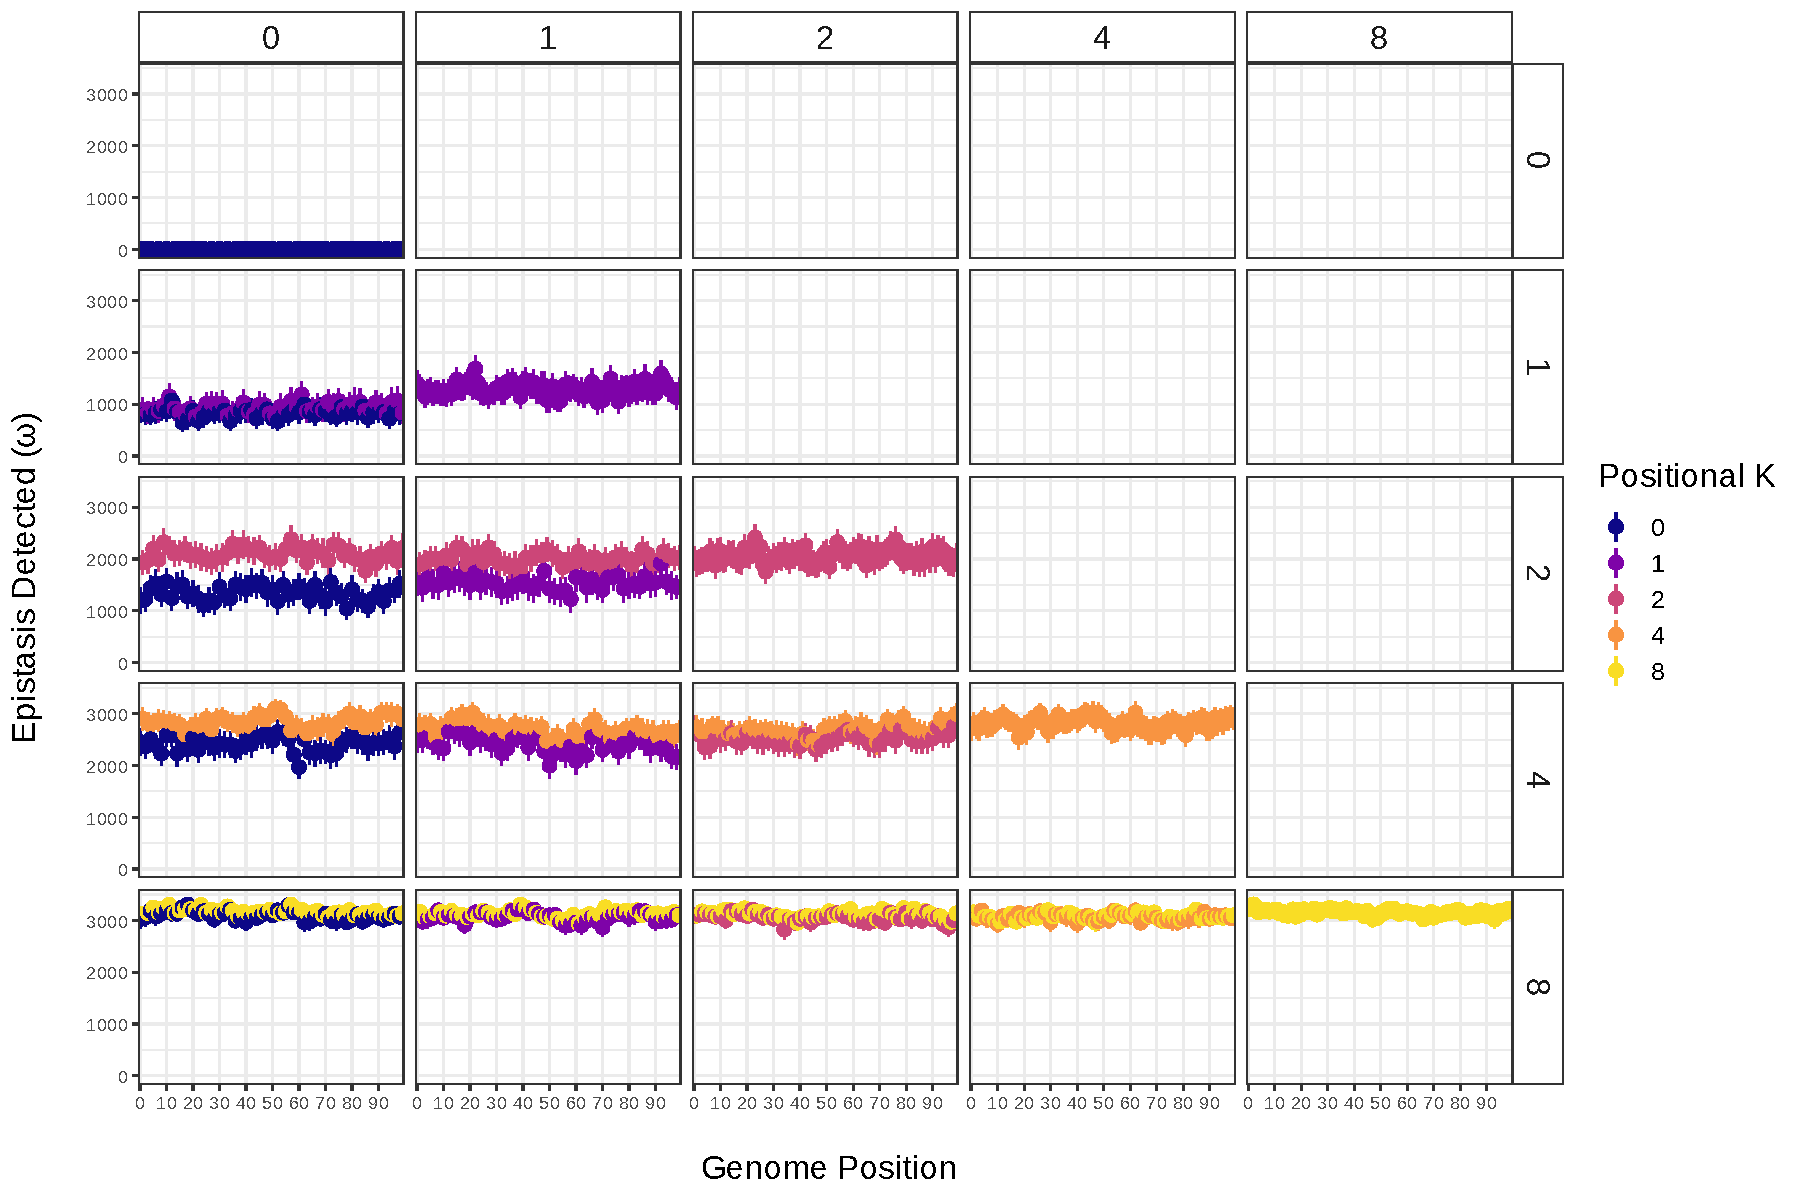
\includegraphics[width=\textwidth]{chapters/1-rank-epistasis/figs/summary_mixed.pdf}
    \caption{Rank epistasis metric $\omega$ on a mixed NK landscape. Top bars indicate the $K$ value set for even-valued. Right bars indicate the $K$ value for odd-valued sites. Each x-axis tick within subplots represents one position in the genome, i.e., the $\omega$ detected for that site. Dots represent mean and bars represent 95\% CIs for 100 replicates.}
    \label{fig:res:mixed}
\end{figure}

In the Mixed landscape, separation of $K$ values is less clear. As the higher $K$ increases, the difference in $\omega$ between lower and higher $K$ values generally decreases; one exception is in the comparison of the mixed $K=0/K=1$ landscape vs. $K=0/K=2$ landscape (Fig~\ref{fig:res:mixed}). 

It is likely that the overall effect of reduced separation of $\omega$ is due to a similar effect as described in the results for the canonical landscape; since evaluation takes place across multiple landscapes, the highly rugged landscapes for large $K$ dominates the level of perturbation detected. In fact, $\omega$ here can be seen as a measure of the ``true" $K$ for each site, as odd- and even-valued sites are \textit{evaluated} on landscapes of different values for $K$ but \textit{interact} with the same number of adjacent sites due to overlap. 

This measurement of ``true $K$" also explains the behavior in the landscapes with $K=0/K=1$ compared to $K=0/K=2$. In the former case, each site where $K=1$ directly interacts with a site where $K=0$, bringing the true interactivity of every site to $K=1$. In the latter case, evaluating every other site with $K=2$ causes the $K=0$ sites to fall completely inside the evaluation block, and interact with only one of the $K=2$ sites at a time. In higher $K$ the landscape staggering does not match the size of the evaluation block and the effect is lost.
